\section{Data}
\label{sec:data}
Luminous red galaxies (LRGs) are massive galaxies that occupy massive halos, lack active star formation, and are considered as one of the highly biased tracers of large scale structure. Redshift of LRGs can be easily determined from  a break around 4000 \AA~in their spectra. LRGs are widely targeted in previous galaxy redshift surveys \mr{(see, e.g., Eisenstein et al 2001, Prakash et al 2016)}, and their clustering and redshift properties are well studied \mr{(see, e.g., Reid et al 2016)}. DESI is expected to collect spectra of millions of LRGs covering the redshift range of $0.4<z<1.0$ over the span of its five year mission. Targets for DESI spectroscopy are selected from imaging surveys; The ground-based surveys that probe the sky in the optical bands are the Mayall z-band Legacy Survey using the Mayall telescope at Kitt Peak \mr{(see e.g. Dey et al. 2018)}, the Beijing–Arizona Sky Survey using the Bok telescope at Kitt Peak \mr{(Zou et al. 2017)}, and the DECam Legacy Survey (DECaLS\mr{;Flaugher et al. 2015}) on the Blanco 4m telescope. Additionally, the Legacy Surveys program incorporates observations conducted from the same instrument under the Dark Energy Survey  \mr{(Dark Energy Survey Collaboration; Fermilab \& Flaugher 2005)}, which constitutes for about $1130 \deg^{2}$ of their southern sky footprint. The BASS+MzLS footprint can be distinguished from the DECaLS by applying DEC $> 32.375$ degrees, although there is an overlap between the two region for calibration. 

\subsection{DESI Imaging DR9 LRGs}
We use photometric LRGs selected from the DESI Imaging Surveys Data Release 9 \citep[DR9;][]{dey2018overview} using the selection designed for the DESI 1\% survey \mr{(Dawson et al 2022)}, described as SV3 in \cite{zhou2022target}. The color-magnitude cuts are described in the $g$, $r$, $z$ bands in the optical and $W1$ band in the infrared, and summarized here in Tab. \ref{tab:ts}. The implementation of these selections in the DESI pipeline is described in \mr{Myers et al (2022)}. DESI-like LRGs are selected brighter than the survey depth limits, and thus the sample density field is nearly homogenous. To further reduce stellar contamination, the sample is masked for bright stars, foreground bright galaxies as well as clusters of galaxies \footnote{See the maskbits at \url{https://www.legacysurvey.org/dr9/bitmasks/}}. Then, it is binned into \textsc{healpix} \citep{gorski2005healpix} at $\textsc{nside}=256$ to construct the density map with an average density of $800$ deg$^{-2}$ with a coverage around \mr{$14,000$} square degrees of the sky. The density map is corrected for pixel incompleteness in the density field of LRGS using a catalog of random points, hereafter referred to as randoms, uniformly scattered over the footprint with the same cuts and masks applied to the DR9 LRGs. 
\begin{table*}
    \caption{Selection criteria for the DESI-like LRG targets from \mr{Zhou et al (2022)}.}
    \label{tab:ts}
    \centerline{%
    \begin{tabular}{lll}
    \hline
    \hline
     \textbf{Footprint} & \textbf{Criterion} &\textbf{Description}\\
      \hline
      \hline   
    &  $z_{\rm fiber} < 21.7$  & Faint limit  \\
          DECaLS & $z - W1 > 0.8 \times (r - z) - 0.6$ & Stellar rejection  \\
     & $[(g-r >1.3)~{\rm AND}~((g-r) > -1.55*(r-W1) + 3.13)]~{\rm OR}~(r -W 1 > 1.8)$ & Remove low-z galaxies \\
     & $[(r-W1 > (W1 - 17.26)*1.8)~{\rm AND}~(r - W1 > W1 - 16.36)]~{\rm OR}~(r-W1 > 3.29)$ & Luminosity cut \\ 
    \hline
    & $z_{\rm fiber} < 21.71$  & Faint limit  \\
 BASS+MzLS    & $z - W1 > 0.8 \times (r - z) - 0.6$ & Stellar rejection  \\
    & $[(g-r >1.34)~{\rm AND}~((g-r) > -1.55*(r-W1) + 3.23)]~{\rm OR}~(r -W 1 > 1.8)$ & Remove low-z galaxies \\
    & $[(r-W1 > (W1 - 17.24)*1.83)~{\rm AND}~(r - W1 > W1 - 16.33)]~{\rm OR}~(r-W1 > 3.39)$ & Luminosity cut \\ 
      \hline
      \end{tabular}
      }
\end{table*}

\begin{figure}
    \centering
    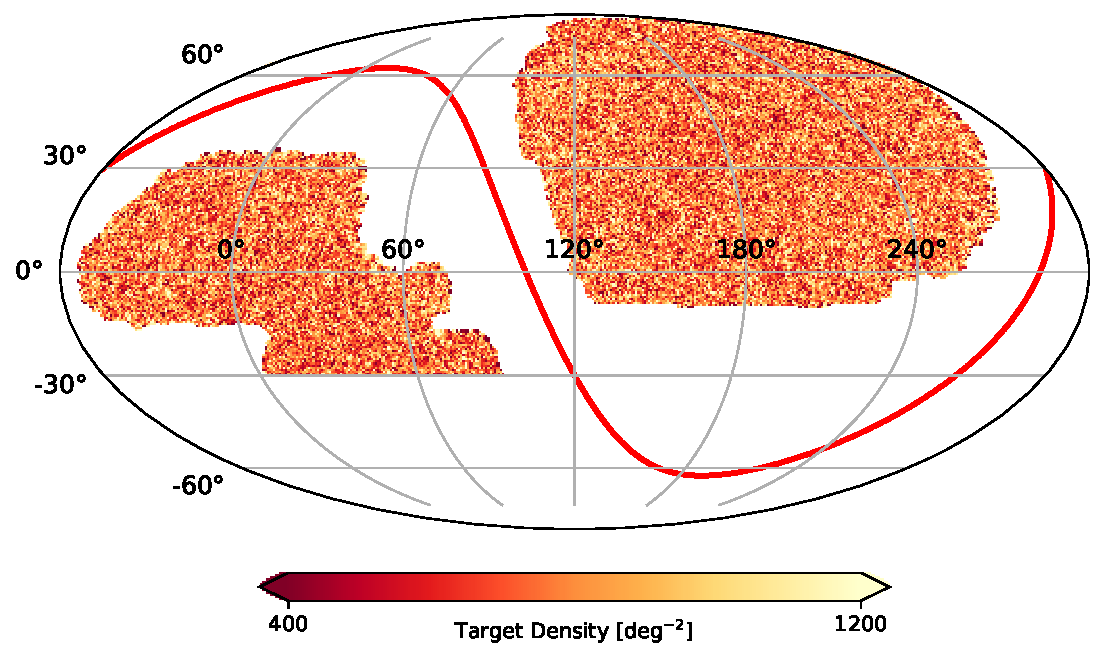
\includegraphics[width=0.45\textwidth]{figures/lrgdens.pdf}
    \caption{Top: Observed density field of DESI Luminous Red Galaxies Data Release 9 \mr{(Dey et al 2018)} in deg$^{-2}$ . Spurious disconnected islands from the DECaLS North footprint at Declination below $-11$ and parts of the DECaLS South with Declination below $-30$ are dropped from the DR9 sample due to potential calibration issues. Bottom: Redshift distribution and bias evolution of DESI LRGs \citep{zhou2021clustering, zhou2022target} \mr{(Zhou et al 2021, Zhou et al 2022, Dawson et al 2022)}. The redshift distribution is deducted from spectroscopy and the bias model assumes a constant clustering amplitude.}
    \label{fig:ng}
\end{figure}

\begin{figure*}
    \centering
    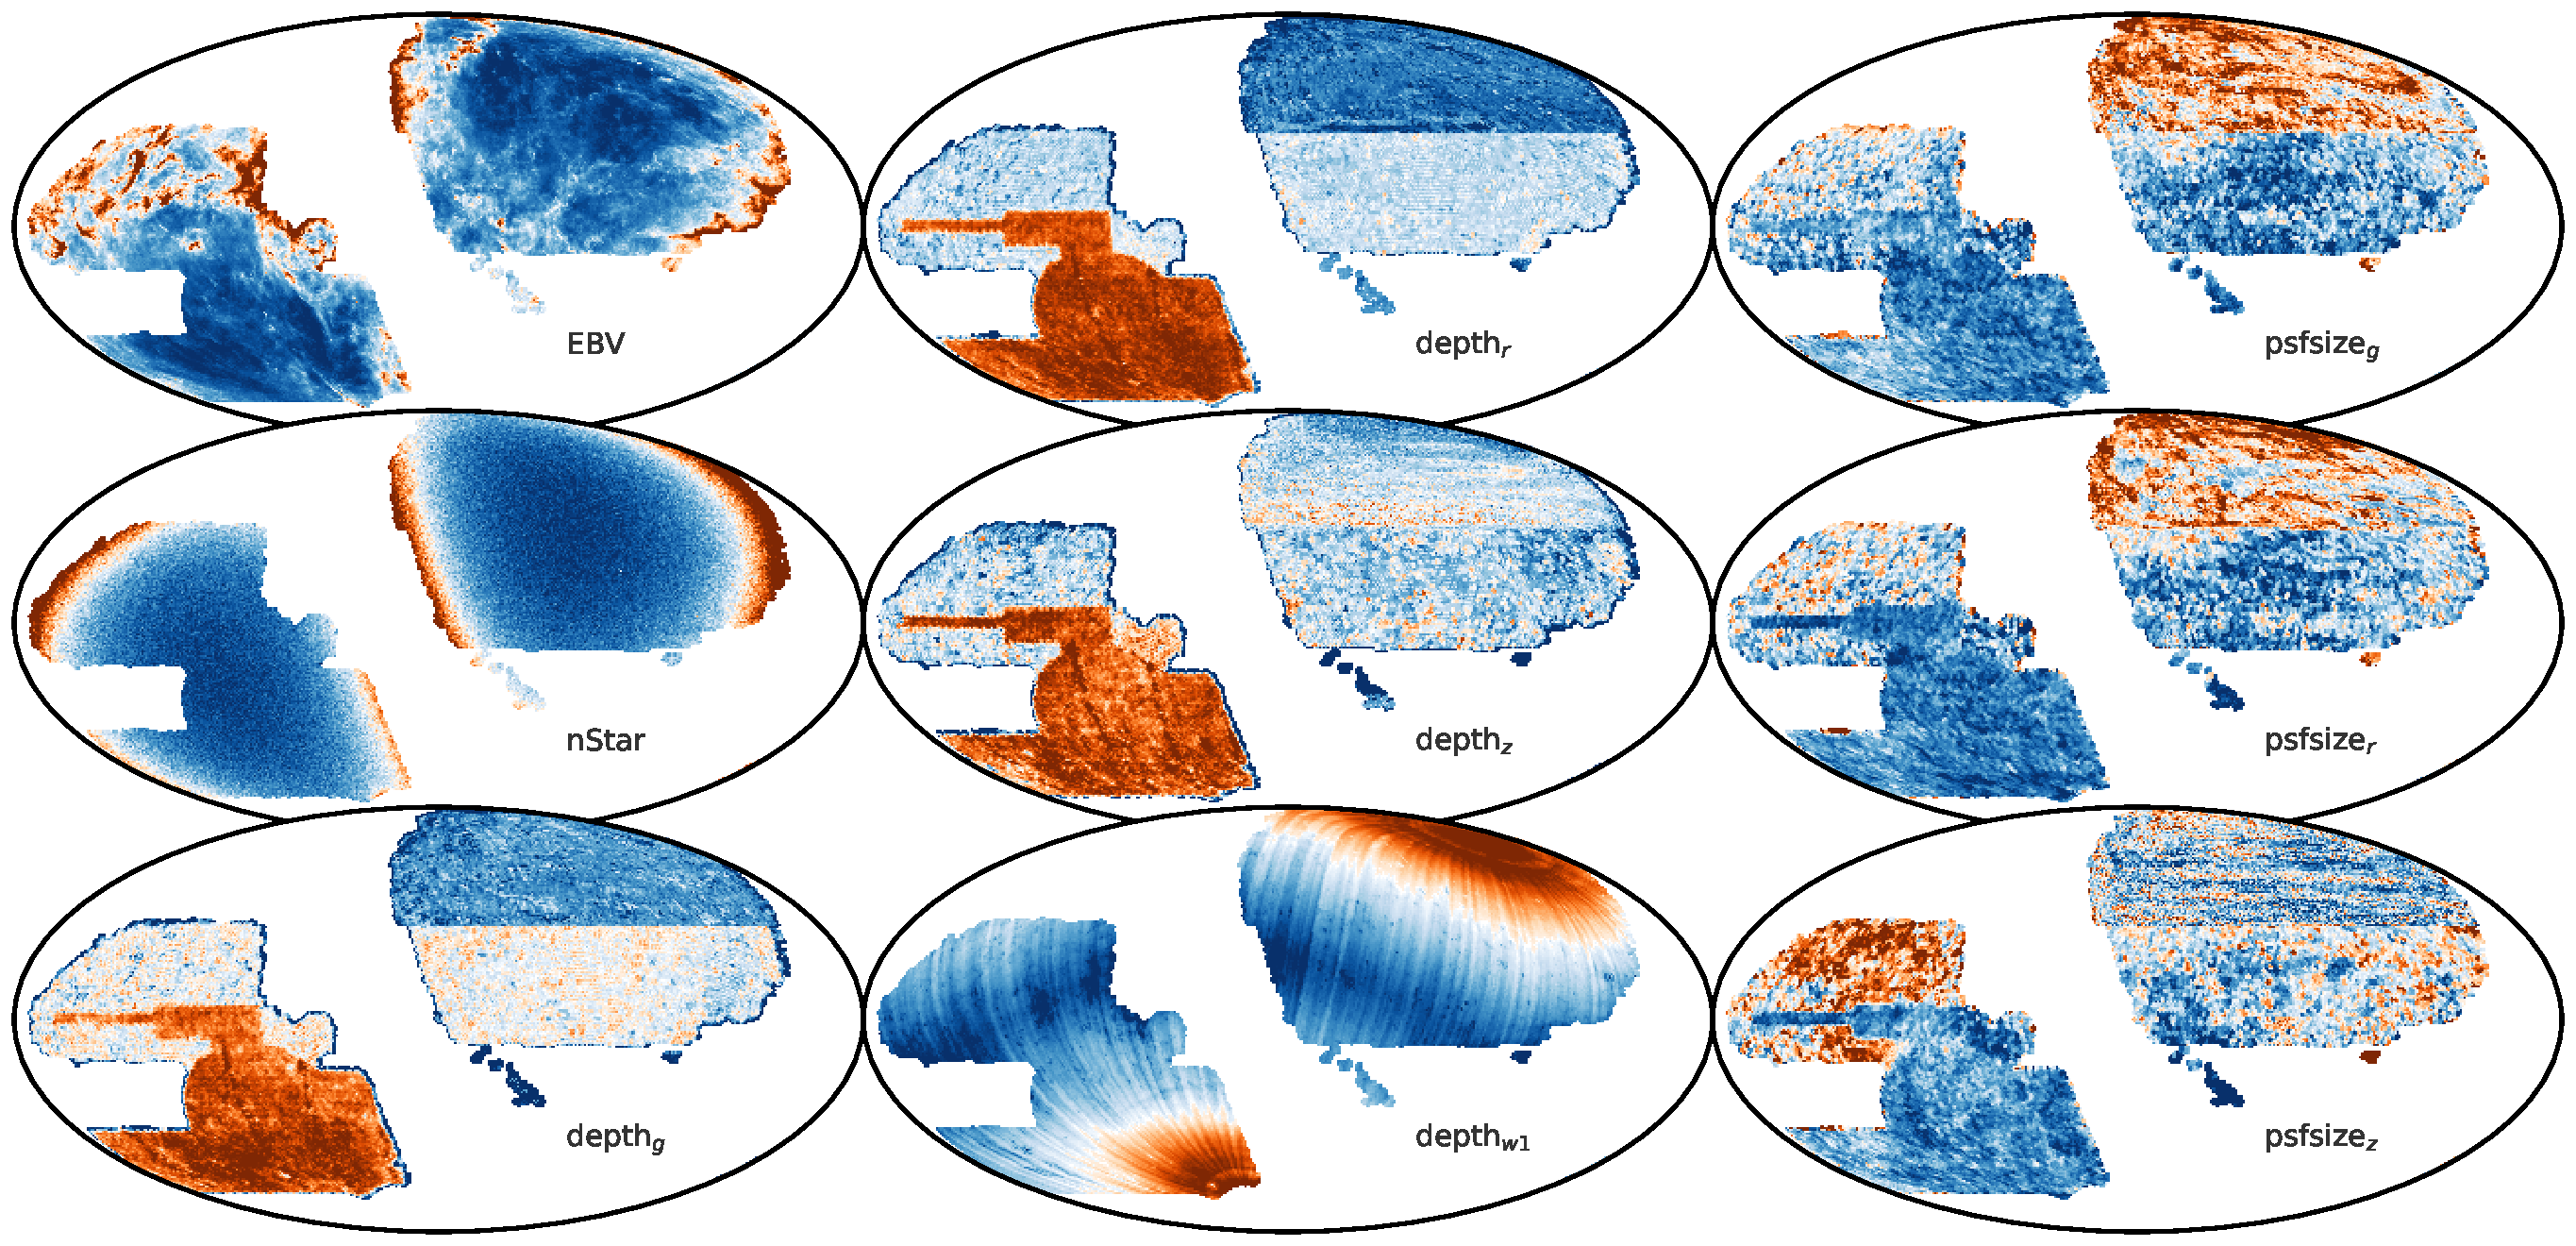
\includegraphics[width=0.95\textwidth]{figures/hp_features.pdf}
    \caption{Mollweide projections of imaging properties in celestial coordinates. }
    \label{fig:xmaps}
\end{figure*}

\begin{figure}
    \centering
    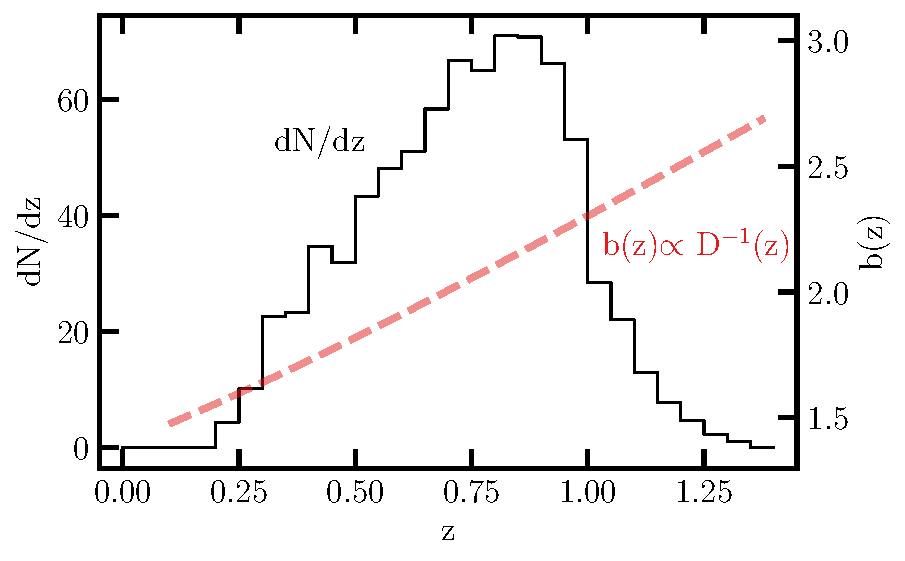
\includegraphics[width=0.45\textwidth]{figures/nz_lrg.pdf}
    \caption{Top: Observed density field of DESI Luminous Red Galaxies Data Release 9 \mr{(Dey et al 2018)} in deg$^{-2}$ . Spurious disconnected islands from the DECaLS North footprint at Declination below $-11$ and parts of the DECaLS South with Declination below $-30$ are dropped from the DR9 sample due to potential calibration issues. Bottom: Redshift distribution and bias evolution of DESI LRGs \citep{zhou2021clustering, zhou2022target} \mr{(Zhou et al 2021, Zhou et al 2022, Dawson et al 2022)}. The redshift distribution is deducted from spectroscopy and the bias model assumes a constant clustering amplitude.}
    \label{fig:nz}
\end{figure}


Fig. \ref{fig:ng} (top) shows observed density field of DR9 LRGs in deg$^{-2}$ before accounting for any potential systematic effects. There are some disconnected islands, hereafter referred to as \textit{spurious islands}, in the DECaLS North region at Declination below $-11$, which are removed from the sample to minimize potential calibration issues. Additionally, parts of the DECaLS South with Declination below $-30$ are cut from the sample, since similar calibration issues might tamper with our analysis. We present  how these data cuts influence our $\fnl$ constraints in Section \ref{sec:results}. Fig. \ref{fig:ng} (bottom) illustrates the redshift distribution of our sample which is inferred from the DESI Survey Validation data \mr{(Dawson et al 2022)}, and the evolution of  galaxy bias for our LRG sample adapted from \cite{zhou2021clustering}, consistent with the assumption of a constant clustering amplitude.

We study the impact of potential sources of systematic error, mapped into \textsc{healpix} at the same \textsc{nside}. Similar to \cite{zhou2022target}, the properties studied in this work are local stellar density constructed from point-like sources with a g-band magnitude in the range $12 \leq g < 17$ from Gaia Data Release 2 \citep[see,][]{gaiadr2, myers2022};  Galactic extinction E[B-V] from \cite{schlegel1998maps}; and other imaging properties include survey depth (galaxy depth in the g, r, and z bands and PSF depth in W1) and seeing in the g, r, and z bands. These maps are produced by making the histograms of randoms (painted with imaging properties) in \textsc{HEALPix} and averaging over randoms in each pixel. Fig. \ref{fig:pcc} shows the Pearson correlation between galaxy density and imaging properties for the imaging surveys in the top panel and the correlation among imaging properties themselves for the full DESI survey in the bottom panel. There is a strong correlation between galaxy density and depth maps and then the second important property seems to be Galactic foregrounds. There is a little correlation between galaxy density and the W1 depth and psfsize properties. We find that there is a large correlation among the imaging properties themselves, especially between the local stellar density and Milky Way extinction; also, the r-band and g-band properties are more correlated with each other than with the z-band. We follow a template based method to derive a set of weights to account for spurious fluctuations by regressing out galaxy counts against a set of imaging maps or templates.  Because of the inner-correlation amongst the maps, a few subsets of maps are considered as well. These subsets are selected to minimize the correlations among the predictors while having maximum correlation with observed density map.
\begin{itemize}
\item Conservative I: Extinction, depth$_{z}$
\item Conservative II: Extinction, depth$_{z}$, psfsize$_{r}$
\item All Maps: Extinction, depth in $grz$ and $W1$, psfsize in $grz$
\end{itemize}
We also investigate whether including external maps for neutral hydrogen column density (\mr{REF}) and calibration (e.g., in the z band; \textit{CALIBZ}) could shed light on remaining systematic effects. 

Linear and nonlinear models (approximated using a neural network) are applied to assess the potential of nonlinear systematic error. Parameters of the models are fit by optimizing the negative Poisson log likelihood, $= \sum \lambda - \rho \log(\lambda)$, where the summation runs over pixels, $\rho$ is the galaxy density, and $\lambda$ is either a linear or nonliner model for galaxy density given imaging properties \textbf{x} as input, $\lambda(\textbf{x}) = \log (1+e^{f(\textbf{x})})$. For finding the parameters of the linear model, we perform a Monte Carlo Markov Chain (MCMC) search using the \textsc{emcee} package \mr{CITE} and for the nonlinear model we use the implementation from \mr{Rezaie et al (2021)}; specifically, the nonlinear model is an ensemble of 20 neural network models. Each neural network is constructed with three hidden layers and 20 rectifier units on each layer. Rectifier is identity function for positive input and zero for negative, and it introduces nonlinearities in the neural network. For the linear model we use all data for computing the log of posterior during MCMC while for the nonlinear approach we use $60\%$ of data for training, $20\%$ for validation, and $20\%$ for testing; this is to minimize the chance of over-fitting by the nonlinear model. By changing the permutation of training-testing splits, we test the nonlinear model on entire data. The training is performed for up to 70 training epochs using \textsc{Adam} optimizer, which is a variant of gradient descent, and the learning rate is tuned on the validation set to dynamically varying between $0.001$ and $0.1$, to enable learning robust against local minima. The best model is then selected with the lowest prediction error when applied to the validation set. Finally, we apply the ensemble of 20 best fit models to the test set and average over the predictions. 

Fig. \ref{fig:npred} shows the predicted density fields from the linear model using various sets of imaging maps, and the nonlinear prediction is also shown for comparison. While most of the large-scale spurious fluctuations are explained by just the extinction map and depth in the z band, adding the psfsize in the r band seems to add more fine structure to the predicted density map. Using all maps does not add much structure. Comparing linear to nonlinear with the same input maps, we find that the nonlinear approach yields finer structure due to a higher flexibility.  Overall, both models predict higher density near the boundaries where the surveys meet the high extinction regions of Milky Way. These regions are probably contaminated artifacts entering the selection either via the direct stellar contamination or the impact of extinction on colors.

\begin{figure}
    \centering
    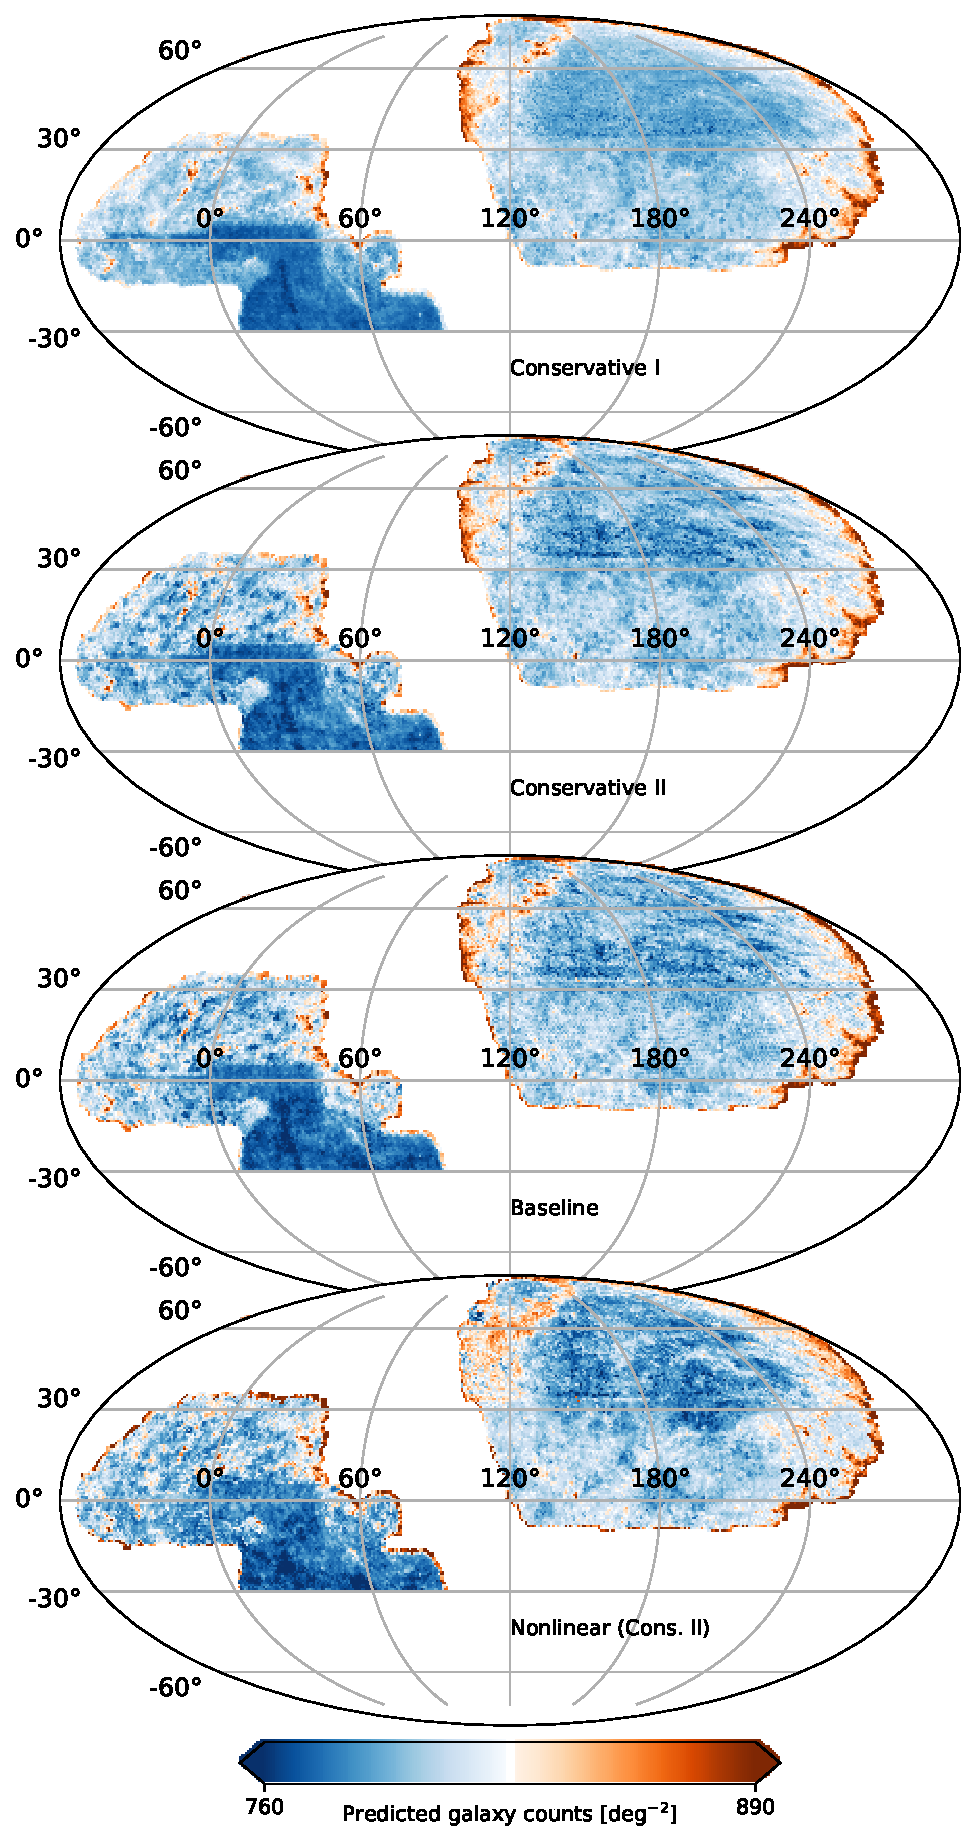
\includegraphics[width=0.45\textwidth]{figures/npred.pdf}
    \caption{Predicted galaxy counts from template regression. Baseline approach uses imaging maps from Zhou et al. (2022): EBV, galaxy depth in rgz, psfdepth in W1, and psfsize in grz. Conservative I uses EBV and galaxy depth in z, and Conservative II uses EBV, galaxy depth in z, and psfsize in r. In all approaches, the models are regressed on BASS+MzLS, DECaLS North, and DECaLS South separately.}
    \label{fig:npred}
\end{figure}

\begin{figure}
    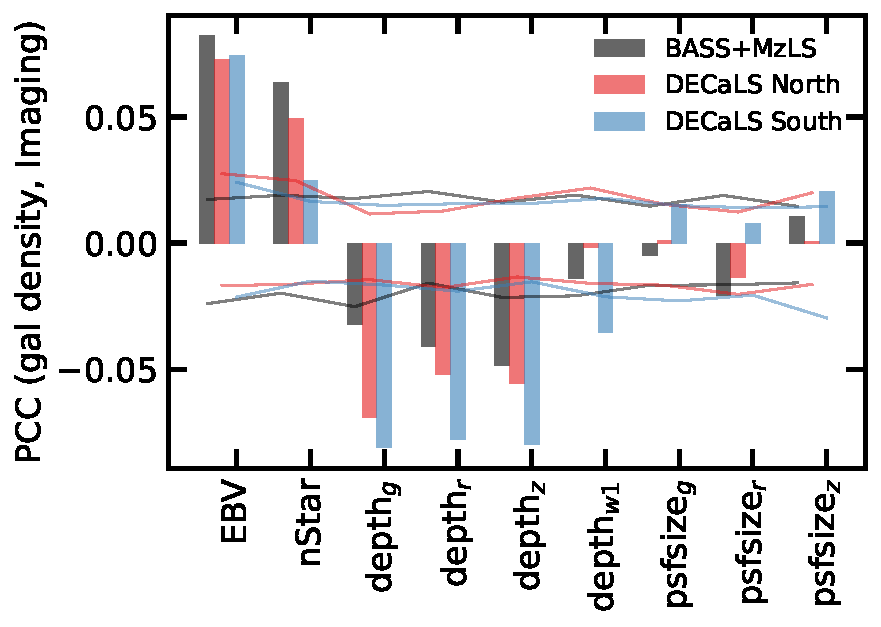
\includegraphics[width=0.45\textwidth]{figures/pcc.pdf} 
    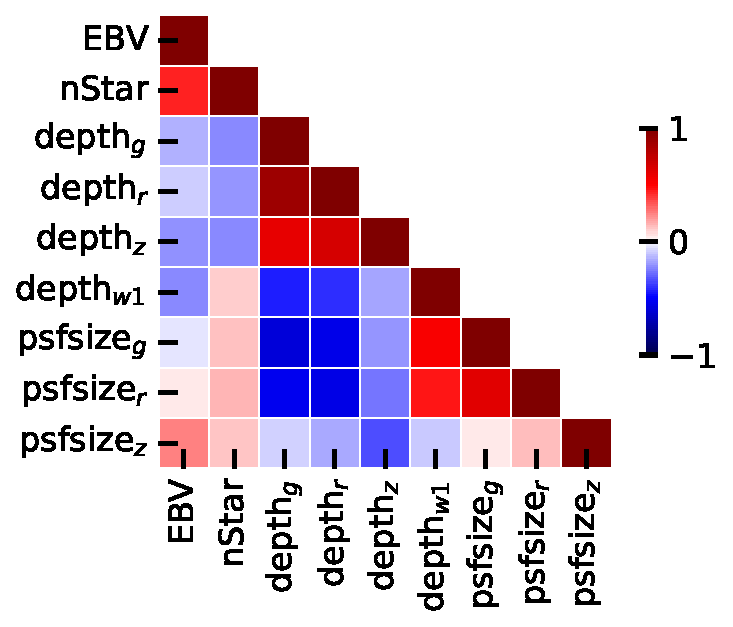
\includegraphics[width=0.45\textwidth]{figures/pccx.pdf}     
    \caption{Top: Pearson-r correlation coefficient between galaxy density and imaging properties in the three imaging regions (top) and between imaging properties themselves for the full DESI footprint (bottom). Solid curves represent the range of correlations observed in 100 randomly selected mock realizations.}
    \label{fig:pcc}
\end{figure}


\subsection{Synthetic lognormal density fields}
Lognormal distributions are shown to be appropriate for describing matter density fluctuations on large scales \citep{coles1991}. Unlike N-body simulations, the generation of lognormal density fields is rather quick and enables a computationaly cheap method to create a large number of realizations, validate analysis pipelines, and construct covariance matrices for error estimation. \textsc{FLASK}  \citep[Full-sky Lognormal Astro-fields Simulation Kit;][]{Xavier_2016} is used to generate series of lognormal galaxy density fields with $\fnl=0$ and $76.92$ using $b(z)=1.43/D(z)$. $1000$ realizations are generated for each $\fnl$. The fiducial cosmology to generate the mocks is based on a flat $\Lambda$CDM universe including one massive neutrino with $m_{\nu}=0.06$ eV, and the rest of cosmological parameters are chosen within $68\%$ of the Planck 2018 resutls \mr{(Planck 2018)},
\begin{equation*}
    h = 0.67,  \Omega_{M}=0.31, \sigma_{8}=0.8, {\rm and}~ n_{s}=0.97.
\end{equation*}
We use the same fiducial cosmology for the analysis of DR9 sample. These parameters are not degenerate with $\fnl$, however the impact of the fiducial cosmology on $\fnl$ constraints is further investigated in Appendix \mr{?}.